%\documentclass[conference,draftcls]{IEEEtran}
\documentclass[conference,final]{IEEEtran}

\usepackage{setspace}
%\doublespacing
%\onehalfspacing

\usepackage{ifpdf}
\usepackage[utf8]{inputenc}
\usepackage{cite}
\usepackage{paralist}
\usepackage[pdftex]{graphicx}
\usepackage{caption}
\usepackage{subcaption}
\graphicspath{{.}{images/}} 
\DeclareGraphicsExtensions{.pdf,.jpeg,.png,.jpg}
\usepackage[cmex10]{amsmath}
\usepackage{url}
\usepackage[rgb]{xcolor}
\usepackage{pdfcomment}

%\usepackage[tight,footnotesize]{subfigure}
%\usepackage[caption=false]{caption}
%\usepackage[font=footnotesize]{subfig}
%\usepackage[caption=false,font=footnotesize]{subfig}
%\usepackage{fixltx2e}
%\usepackage{stfloats}
%
%\usepackage[rgb]{xcolor}
%\usepackage{pdfcomment}

\newcommand{\dme}[2]{\pdfmarkupcomment[markup=Highlight,color=yellow]{#1}{#2}}
\newcommand{\notedme}[1]{\raisebox{0pt}[0pt][0pt]{\pdfcomment[open=true,color=blue]{#1}}}
\newcommand{\todo}[1]{\pdfmarkupcomment[markup=Highlight,color=red]{#1}{todo}}

% \newcommand{\red}[1]{\pdfmarkupcomment[markup=Highlight,color=red]{#1}}
% \newcommand{\green}[1]{\pdfmarkupcomment[markup=Highlight,color=green]{#1}}
% \newcommand{\grey}[1]{\pdfmarkupcomment[markup=Highlight,color=gray]{#1}}
\newcommand*{\bd}[1]{\multicolumn{1}{|c}{\bfseries #1}}


% correct bad hyphenation here
\hyphenation{op-tical net-works semi-conduc-tor}


\begin{document}
\title{Intrusion Detection of a Wireless Sensor Network\\Over the Air Update Protocol}
\author{
		\IEEEauthorblockN{	A S M Ashraful Alam\IEEEauthorrefmark{1},  % and
							David Eyers\IEEEauthorrefmark{1},  % and 
							Zhiyi Huang\IEEEauthorrefmark{1} 
						}
	\IEEEauthorblockA{\IEEEauthorrefmark{1}Department of Computer Science, University of Otago, New Zealand, Email: \{aalam, dme, hzy\}@cs.otago.ac.nz} 
}


% use for special paper notices
%\IEEEspecialpapernotice{(Invited Paper)}

\maketitle


\begin{abstract}
Robotics and  Wireless Sensor Network (WSN) collaborations is an emerging research field in which both the technologies can benefit from integrated implementations.
In this paper, an Intrusion Detection System (IDS) for WSN  software update protocol is designed and simulated. 
The IDS protects WSN software updates that use over the air (OTA) update protocols, specifically the Deluge protocol.
When the protocol modifies the running software in a mote, the mote sends related  information to the sink. 
The IDS in association with an IDS Transport Client (ITC) in the sink analyse the update phenomena of each of the motes in the network and computes a `Intrusion Warning Score' (IWS) through an algorithmic function to indicate a possible intrusion i.e., a probable illegitimate update.
\end{abstract}

%\begin{keyword}
%\kwd{Wireless Sensonrs}
%\kwd{WSN}
%\kwd{Intrusion Detection System}
%\kwd{Security}
%\kmw{Robotics}
%\end{keyword}

% no keywords
% For peer review papers, you can put extra information on the cover
% page as needed:
% \ifCLASSOPTIONpeerreview
% \begin{center} \bfseries EDICS Category: 3-BBND \end{center}
% \fi
%
% For peerreview papers, this IEEEtran command inserts a page break and
% creates the second title. It will be ignored for other modes.
\IEEEpeerreviewmaketitle %not meant to be here for submission
Security of sensed environmental data external to the robots
%ICARA does accept papers on sensors. With collaborative robotics increasing rapidly, security of inter-robot communication over wireless media is of great importance. Your proposed paper would be of interest to ICARA attendees and we look forward to receiving your paper by 27th October.

\section{Introduction}
\label{sec:intro}
%	\subsection{Subsection Heading Here}
%		\subsubsection{Subsubsection Heading Here}

%\subsection{Application of Sensors in Robotics. How important is WSN in robotics}
Wireless Sensor Network (WSN) has attracted many robotics researchers because of the potentials for many problem solving applications, such as robot localisation, path finding, sensing, mapping. 
The wireless sensors and robotics can be coined to offer great advantages in many fields like ambient assisted living, environmental monitoring, vine pruning, and so on.
Mission critical robotics applications in military, mining industry, team collaboration, or companion for older adults employ wireless sensors as well.
Conversely, robotics can be utilised to solve WSN problems like sensor deployment/relocation in hostile environment, data aggregation, acting a data mules.
Connecting WSNs with group of robots can extend the capability of each other.
Integrated WSNs and robotics applications augment a robot's interaction and decision making capabilities and services where WSNs can be deployed in the environment.

Devices in WSN are known as nodes or motes, are generally self-powered with inbuilt limited processing hardware.
A mote has an embedded microprocessor, a radio and one or more sensors.
The manager node, which is connected to a workstation with greater processing capability is called a sink or base station. 
All sensor nodes in a WSN has an unique identification number called `Node ID'.
Motes and sinks, using the same radio channel and protocols,  dynamically form an autonomous networked environment where all sensor nodes within range take part.
Data exchange in WSN takes place only locally using an autonomous relay mechanism that does not have any routing table. 
A WSN is ultimately employed for sensing and detecting certain physical phenomena, on which basic processing is performed at the individual mote, the processed information is relayed back to a computing device  through the sink for further processing.
WSNs are generally deployed for long-term monitoring at scales and resolutions that are difficult to manage. 
They may necessitate reprogramming after deployment to accommodate alteration in the environment, sensing applications, or scientific requirements~\cite{ISI:000253439700120}.
The update time is the time when any mote begin executing a new version of the software image.

%\subsection{What is intrusion}
Intrusion is an illegitimate act that aims to disrupt or degrade the intended functionality of the network or a part of it; it  may or may not be intentional.
Intrusion in software update primarily means uploading inappropriate software that performs undesired actions, clandestinely replacing the  sensor operating system (OS) software, and so on.
An intruder may also prevent the update propagation, waste network resources, disrupt the normal operation of code dissemination, inject malicious codes to pollute the network and deny intended function by  injecting bogus or modified software or updates. 


Sensors have huge limitation in their capability to be independently useful.
Sensors can sense, they cannot react. 
They have resource constraints like with respect to processing power, tiny memory, storage, and severe energy.
The motes are not suitable for heavy computational tasks.
On the other hand, robots have greater capabilities like mobility, performing resource intensive tasks, operating in unfavourable environments.
Combining the capabilities of WSN and robots are therefore very conducive in a unified fashion.


Reprogramming of the sensors is one of the most important management tasks.
It is not easy to round up all the deployed sensors in order to reprogramme them. 
Hence automatic over the air (OTA) reprogramming of sensors becomes an important issue.
OTA software update poses two main security challenges: maintaining confidentiality and integrity of data. 
An attacker quite easily may pickup and read the motes deployed in the environment.
Similarly, he can inject false data into the sensor that can infect the network using epidemic protocols. 
Thus, adding wireless sensors add additional security challenges in robotics.



%\subsection{Security of WSN and Update needs. what are the problems. }
Software update in WSN is a vulnerable process.
It implies effects beyond the updates only.
The process is particularly vulnerable because the running OS and application need to switch from old version to new one. 
At one stage during this process, security  measures on the sensor motes are deactivated or unavailable for a short period of time.
This opens up a vulnerable window in time when it is easier to intrude.
From network point of view, the update process contributes to a significant increase in traffic that an adversary may exploit to  mask his actions. 


%An IDS architectures for static WSNs has been suggested that watches over the communications in the neighbourhood . Such an IDS is not capable to identify a malicious update that has been effected by an adversary in the WSN.

%Data dessemination protocols
Several OTA network data dissemination protocols for WSNs have been implemented, which target at attaining efficiency, throughput and conserve energy.
They generally do not cater cryptographic protection for source authentication, integrity verification and likewise. 
The program binary authentication technique using a hash is not very useful in to resource-constrained sensors. 
Deluge, which is a protocol for disseminating data objects in the network, uses density aware epidemic property for its operation \cite{1031506}. 
Deluge incorporates digitally signed initial advertisement  and authenticated broadcast scheme. 
However, we contend that it is possible for a malicious intruder to replicate an authentic image source and advertise new programme version which the motes cannot repudiate. 
Even though,  Deluge incorporates on-chip hardware based encryption,
Cryptography alone cannot completely prevent attacks. %on WSNs confidentiality, authenticity, availability due to resource limitation.
Constrained computational capacity and resources make it possible to compromise the cryptographic measures incorporated in the implemented WSN OSs.
The other vulnerability of such epidemic protocol is breach at any one point does the job of weakening the whole network for the attacker. 
An attacker may appear somewhere in the network, pretend to be an authentic source and disappear after successful introduction of the illegitimate image to one mote in the network. 
The security mechanisms provided by Deluge would be unable to detect the initial breach in such cases and would allow the network to be flooded by a totally new version of the application that performs completely different function~\cite{Karlof:2004:TLL:1031495.1031515}.
While the reprogramming protocols are essential for the WSNs, they could act as carriers of rapid spread of malicious code in the network.


%\subsection{Why WSN communication in robotics/any application need to be secured. }
%If inputs from wireless sensors are forged, then catastrophic errorneous results are expected			
%\subsection{Why it is important to secure updates? How WSN updates can be forged to impede the capabilities of robotics}
Security is one of the major concerns for adopting WSN technology. 
Keeping WSNs secure is a challenging task because of the wireless environment and possible  wide variety of applications.
Security techniques developed for other wireless technologies cannot readily be employed in WSN for the limited resources.
A robot may be fed with wrong kind of stimuli from the environmental WSN sources that might  lead to undesired robotic responses. 
Various possible attacks on WSNs have been explained in~\cite{roosta2006taxonomy}, \cite{roosta2008attacks}.



%\subsection{Why it is necessary to have IDS not encryption in case of WSN}
Security schemes in WSNs have two main approaches --- using cryptography (crypto) to secure communication and  employing Intrusion Detection System (IDS) to oversee activities.
Crypto techniques are active approaches through use of cryptographic keys, encryption and decryption schemes, algorithms, policies and procedures.
Because  of the absence of the session and presentation layers, and resource constraints, designing crypto based security solutions for wireless sensors are complicated, expansive and often may not be effective.
An adversary can employ much greater computing resources to break in through the protection provided by crypto solutions.
Moreover, absence of switches and gateways in WSN hampers monitoring of information flow.
Thus it is useful to employ some passive security measures alongside crypto solution.
An IDS detects suspicious behaviour in the network, provides useful information like identification and location of the intruder, extent of intrusion and likewise.

%\subsection{Lit Review} % Heading to be commented out
Despite the need of huge security research in WSN, only few previous studies have considered IDS approach in recent years.
An anomaly based IDS approach that works in a distributed manner and uses support vector machine to minimise communication overhead while performing in-network anomaly detection has been proposed by~\cite{ISI:000257882502160}.
A standalone rule based approach to detect anomalies at all layers of a network stack in WSN has been suggested by ~\cite{ISI:000232429900067}.
Rule based  techniques rely on monitoring of group of nodes and routing tables for detection~\cite{ISI:000298891500099, Chen:2009:NMI:1516241.1516282, 1424814, Strikos_afull}.
On the other hand, spontaneous watchdog technique uses the sensor broadcast, density of deployed sensors for its detection~\cite{1593102}.
Specification based  IDS has been proposed that relies on data clustering and uses standard deviation from the average inter-cluster distance~\cite{Chen:2009:NMI:1516241.1516282, 1424814, Strikos_afull, 4085803}.
 
Statistical based anomaly  detection looks for anomalies in routing pattern~\cite{4024996}.
A serious weakness with this methods, however, is that  it uses hidden Markov model to focus on the accuracy of the gathered data, rather than the security of the nodes or the links~\cite{1290173}.
The model monitors data arrival process in real time traffic on the nodes, analyses short term dynamic statistics using a multi-level sliding window event storage scheme.% that works on each node. 
The detection algorithms performs locally and individual nodes are not aware of the network-wide attacks~\cite{1515559}.
In contrast, some other statistical procedures exploit the stability of the neighbourhood information of the WSN nodes depending on average receive power and average packet arrival rate~\cite{1512911}.

Game theory based IDS utilise Markov chain for its decision making process can monitor only one of the clusters of the network at a time, which leaves the rest of the network unprotected~\cite{1347798}, \cite{Das07preventingdos}, \cite{Reddy:2009:GTA:1607720.1607944}.
Reputation based IDS relies on heuristic ranking algorithms to identify most likely bad nodes in the network.
Such IDSs use high scalable cluster-based hierarchical trust management protocol to effectively identifying the selfish and malicious nodes~\cite{6174485}.

Although very good results have been obtained from some of the approaches described above, only few of them are able to specifically address the security issues related to software update in WSN.
The security countermeasures available in WSN systems is predominately cryptographic.
The WSN OSs do not incorporate an IDS approach due to the reality that such an employment would cut down on the resources, especially power.
An IDS residing on the sensors is ideally need to be avoided by design.

Hence, we propose an analytical tool that sits outside the network and yet can have valuable insight into the propagation characteristics of OTA reprogramming protocol. 
%The tool should be flexible for comparative studies of different protocols. 
The tool, which is essentially an IDS, can primarily be applied on OTA protocol.
The technique has been tested on Deluge.
We have exploited services from other existing standard protocols a to gather timing information outside the WSN and then process the timing information for intrusion detection.
Use of timing analysis approach is a novel technique in IDS for WSN.
%The technique may further be extended for use with broad range of intrusion detection motives specially in WSN and also in MANET.
The technique is centrally controlled, resides outside the WSN, gathers processed information from the sensors in WSN.
%However, an IDS with that broad spectrum is out of scope of this paper.
%We shall limit ourselves within its application on WSN, specifically on Deluge only.
%Before one understands how the IDS works and is able to focus on its  mechanism, one needs some prior knowledge about Deluge and its security techniques.
The IDS identifies the anomaly in software update pattern in terms of quantitative score. The higher score indicates a higher probability of intrusion at some point in the WSN. The score can be deterministically classified when some additional information is available.


%\subsection{How do I plan to handle them (How do I do it). > Contributions} \\
A suitable IDS can detect  break in events. 
However, an IDS does not prevent the break in, but alerts following some predefined procedures in case of a security breach.
Research in WSN security with respect to IDS has lots of potentials for new discovery and implementation. 
We propose a novel algorithm that requires minor modification of the OTA update protocol by incorporating Active Message (AM). 
AM is a single-hop, unreliable packet used for network abstraction in TinyOS. 
It has a destination address, a type field, provides synchronous acknowledgements~\cite{tep116}. 
AM equips the IDS with a centralised view of a network-wide knowledge that is processed and analysed to work out a score function according to indicate a possible intrusion.
This work's contributions are two fold.
\begin{inparaenum}
\item  The IDS identifies anomalies in software update patterns and scores them quantitatively;
\item The scheme i.e., the IDS expectations can provide useful insight for designing secure WSN.
\end{inparaenum}
%% <Ashraf> is this paragraph a repeatation of the previous one. But there are some useful info here


%\subsection{Organisation of the paper }
The rest of this paper is structured in the following way. 
%In Section~\ref{sec:lit}, we provide an overview of intrusion related research works in WSN software update protocols. 
%We look up for  security aspects not addressed by the present WSN security researchers and the reasons behind any security deficiencies. 
In Section~\ref{sec:meth}, we describe the experiment methodology and an overview of the system  design. 
We then present the findings from the experiments, analyse the result and present our evaluation in Section~\ref{sec:eval}.  
Finally, we conclude our arguments in this Section.




%%\subsection{WSN and robotics works and what they mainly address and what they do not}
%% <Ashraf>  What to do with this paar
I DONT KNOW IF I WANT TO KEEP THIS PARA.
Mobile robot navigation is an emerging research field where robotics and wireless sensors collaborate.
Nodes in WSN can greatly enhance the perception capabilities of robots with robust communication coverage.
Security is one of the main concerns in such collaborative approach.
There are security issues with use of cryptography in WSN due to the nature of the hardware~\cite{1710}.
Usually, an IDS detects suspicious behaviour in the WSN.
Butun, Morgera, and Sankar authoritatively discussed the constraints and challenges in WSN IDS design~\cite{6517052}.
An IDS can use distrbuted , cooperative architecture with a hierarchical or centralised approach.


\section{Methodology}
\label{sec:meth}
In this section , we describe the study environment, procedures, and the design of the system.
%It's helpful to both writer and reader to organize this section chronologically: that is, describe each procedure in the order it was performed. For example, DNA-extraction, purification, amplification, assay, detection. Or, study area, study population, sampling technique, variables studied, analysis method.
The proposed IDS and its techniques were evaluated in comprehensive simulations.
While the system has been elaborately designed and aimed at testbed evaluation, it has not yet been performed at this stage of the research. 
%The testbed implementation will be evaluated at some point in the future.
The simulation environment possessed the ability to observe the software update pattern in a fully functional WSN where each node generates and reports the time at which the new software update completes and starts executing.
The raw data generated from simulation logs were processed, related and  analysed to produce the IWS.

\subsection*{Simulation Environment}
\label{subsec:sim_env}
The IDS requires Deluge protocol to be able to report the time of executing  a new version of its software.
The protocol was originally implemented in TinyOS and later has been ported to other embedded operating systems including Contiki. 
We used Deluge protocol implemented in Contiki v2.7 on a system running on Ubuntu 12.04.
%[So this will eventually need citation and a self-contained description.]
`Cooja', a network simulator for Contiki, was used to simulate the software update pattern associated with Deluge protocol. 
%We also used a plugin for Contiki called Mobility to aid our experiential setup.
%Although the plugin was designed to deal with positions over time for the nodes in the simulation, we used it to load the exact location of the sensor motes into the `Cooja' simulator. 

\subsection*{Design of Experiments}
\label{subsec:exp_des}

The simulations were cautiously designed and planned to evaluate the proposed IDS in different topologies and variable parameters like power level.
Evaluating the IDS on each of the topologies consisted of several test runs.
The test runs were of two kind: 
\begin{inparaenum}
\item Test runs aimed as establishing baseline data consisted of 20 individual simulations which were initiated from the sink; and
\item Simulations that replicated an intrusion at different points of the WSN were initiated once from each of the nodes except the sink.
\end{inparaenum}
Results obtained from all these simulations were utilised to model the expected pattern for a particular topology.

\subsection*{Topologies}
\label{subsec:topos}
The topologies were designed based on different design considerations that were established using number of trial and error test runs to meet specific requirements like shape, distance, range and power level. 

\begin{table*}[t!]
\centering
\begin{tabular}{|l|*{8}{r|}r}
\hline
\bd{Topologies}           & \bd{Linear} & \bd{Circular} & \bd{Elliptical} & \bd{Double Rings} & \bd{Wide Line} & \bd{Grid} & \bd{Tree} & \bd{Owheo WSN}   \\
\hline
\bd{Number}           & 20 & 20 & 20 & 46 & 45 & 72 & 25 & 37   \\
 \bd{of Motes}           &  &  &  &  &  &  &  &    \\
\hline
\end{tabular}
\caption{Number of motes used in each topological deployment}
\label{tab:topos}
\end{table*}

%The shape of the experiential topologies were designed as linear, circular, elliptical, double rings, wide line, grid, tree and other random topologies.
%The names of the topologies here indicate that in each case the motes were deployed along the circumference of the geometrical shape that enabled packet propagation to take place according to a designed fashion.\notedme{drop---too obvious to justify saying.}
%In each topology, minimum 20 nodes were deployed for a test to take place. 
%More motes were necessary to replicate certain topologies.
Table~\ref{tab:topos} shows the number of motes used in experiments in corresponding topological  deployments.
The motes were placed at a distance of 30--35 meter to allow  multiple transmission paths to all the motes along the circumference of the intended topological shape. % <dme> en-dash for number ranges, not em-dash	% <ashraf> I am trying to increase my English and LaTeX vocabulary
For most experiments, the radio transmission power level was set at 100\% which has an approximate maximum effective transmission range of 50 meter and is able to interfere other motes upto 100 meter away.
The Owheo WSN topology was additionally tested at 50\%  to quickly observe the difference from the parameter change.


\subsection*{Procedure}
\label{subsec:proc}

Experiment procedure  was a combination of activities such as running simulation, analysing system log and processing data to arrive at a conclusion. 


\subsubsection*{Processing  of Individual Test Run}
\label{ssc:test_runs}
%Step 1: Running simulation
In the environmental set up described above , all motes in the WSN were booted up at same time running one version of a diagnostic application. 
The diagnostic application would necessarily report its time, version number and mote ID on the serial terminal every second at its serial port. 


%Step 2: Stopping the simulation
The base station dynamically began the update process and propagated another version of the software (also called image) using Deluge protocol. %, which is also called 
Whenever new image transfer to a mote was complete, the image would replace its old version and reboot to begin executing the new one.
The new application also necessarily allowed the motes to report their time, version number and mote ID on the serial terminal. 
The simulator continued until all the motes in the WSN were updated and the reported events were logged. 
%Step 3: Filtering out mote update time and distance
The update time of each mote were filtered out  and were sorted In ascending order of update time.

%Step 4: Calculating the euclidean distance and sorting
%A cpp application was used to take input from this semi-processed information and another file that preserved the position information of the motes in the deployment.
%The application processed the data to find out the euclidean distance of the motes from the sink.
%It additionally sorted the rows based on update time in ascending order.
%At this instance, we preserved the processed information in a file in following fashion:
%\begin{verbatim}
%--------------------------------------------
%| 	Time (in ms)	|	Mote ID	| Distance |
%--------------------------------------------
%\end{verbatim}

%Step 5: Calculating baseline data
\subsubsection*{Building the Baseline Data}
\label{ssc:build_baseline}
Processed data from 20 simulations, initiated from the sink, were considered for each topology.
Any change in variables in the environment or in the topology would necessitate recalibrating the baseline.
Mean and standard deviation of mote update times were statistically calculated to build the baseline.
These were the inputs to the IDS to calculate the IWS according to the utility function shown in Equation~\ref{eqn2}. 

%Step 6: Calculating IWS
\subsubsection*{Calculating IWS}
\label{ssc:calc_iws}

Intrusion attacks at different nodes were replicated in simulations.
The individual simulations runs were treated in a fashion  similar to~\ref{ssc:test_runs}.
The update time recorded at each of the motes were mathematically treated according to the utility function in Equation~\ref{eqn2}, which performed the following computations:
\begin{itemize}
\item Subtract the new update time from the corresponding mean of reference update time for each of the motes to calculate the absolute difference. For example, new update time of updated mote `$n$'(new) is subtracted from mean update time found from the baseline data for mote `$n$' and its absolute value was calculated.
\item The absolute difference is divided by a function of standard deviation to avoid any `division by zero' scenario. This also smooths the data to avoid unrelated variations.
\item Sum up the resulting scores at all individual nodes in the WSN to find out the total IWS for the update.
\end{itemize}
The resulting numbers  presented an approximation of abnormality of the new update pattern. The higher the score, the more dissimilar was the pattern. 

\subsection{Overview of the System}
\label{sec:des}


\subsection{Threat Model}

%What are the security aspects it does not handle?
%Why does not it handle them?

The threat model is directed towards injection of unauthorised program image to infect the entire WSN.
The IDS is also expected to handle malicious node update, node compromise, node failures.
In addition to this, the IDS also considers a threat model where a new node pops up and injects the new software image by compromising existing WSN security mechanism.

%The main threat scenario that the IDS is expected to handle is compromise of a particular node in the WSN and then attacker being able to utilise the same node or replicate the node to inject a new software image using Deluge protocol in the WSN.
%However, once the new image transfer has been injected, the node may remain alive or disappear.
%In case the compromised mote disappears, WSN would consider it as a node failure instead of node compromise.
%Actually, the node was hijacked to infect the WSN and create more confusion in determining how the incident took place.
%\begin{itemize}
%\item Node failure
%\item Node compromise
%\item Malicious node update
%\item Popping up of intruder node
%\end{itemize}

%Cases that it cannot handle. 
The IDS cannot identify an intrusion in certain scenarios.
For example, when an intrusion takes place in close vicinity of the sink, this IWS may not always be significantly large to be identified as an intrusion. 
%Moreover, due to node compromise in one of the motes and intrusion initiated from another mote may result into unsurprising score due to fact that the effects may cancel each others contribution to the score.
The deployment should consider additional security measures to handle such scenarios.


\subsection{Assumptions} %Should I put it here or in discussio section.
\label{sc:assump}

%Assumptions that are discussed in-text are discussed in the context of the limitations of your study, which is typically in the discussion section. This is important, because both assumptions and limitations affect the inferences you can draw from your study. - See more at: http://phdstudent.com/Choosing-a-Research-Design/stating-the-obvious-writing-assumptions-limitations-and-delimitations
%The system is expected to achieve a time synchronisation. 
%That's entirely reasonable, but it needs to be stated as an assumption about the WSN under study.
%I AM NOT SURE IF THIS PART IS AN ASSUMPTION> THIS IS A FACT.


The paper assumes several WSN settings and capabilities.
One of the most important assumption is: there is only one sink in the network. While WSN with multiple sinks are also possible, the IDS needs to be designed differently and are have not been studied at this stage of the research. 
It further assumes that the sink is protected from all kind attacks and cannot be compromised. 
The system do not consider mote mobility scenario and assumes a static WSN.
%The system operates in a fashion that whenever a new image updates a mote, it sends an AM to all the base stations in the WSN, thus the software update behaviour in the WSN is transparent to the IDS.

%The IDS is aware of the topological information that has been setup in the WSN.
%It knows the location of all nodes deployed in the network.
%I AM NOT SURE IF IT SHOULD COME AS ASSUMPTION. THIS IS ALSO A DESIGN ISSUE.
%However, assuming software update behaviour in the WSN transparent to the IDS enables fixing the scale for triggering warning.

%\begin{itemize}
%	\item	The WSN is of homogeneous nature and works in the same network.  - Too obvious
%	\item 	All motes in the WSN runs same version of the software.  - Too obvious
%	\item	IDS resides externally.  - A design issue, not an assumption
%	\item	There is A single sink in the WSN. 
%	\item	The sink is protected and cannot be compromised.
%	\item	Whenever possible, there are more than one route to reach each of the motes
%	\item	The WSN is static in nature- All motes in the WSN are static.
%	\item	Whenever a new image is updated in a mote, it sends a conformation active message to all base stations in the WSN, thus The software update behaviour in the WSN is transparent to the IDS.
%\end{itemize}

%\subsection{Algorithm}
%\label{subsec:alg}
%NOT STATED / DISCUSSED IN THIS PAPER\\
%This is a part in the original thesis though.



\subsection{System Design}
\label{subsec:sysdeg}


The proposed IDS resides on a computing system that is physically connected to the sink.
It relies on existing protocols for its operations.
Related information is collected utilising standard transport layer protocols. 
The IDS analyses the update time of  each of the motes in the WSN and computes a `Surprise Score' or `Intrusion Warning Score' (IWS) using utility function in Equation~\ref{eqn2} and indicates the cases of a possible intrusion, i.e., a probable illegitimate update.

The intrusion detection algorithm suggests some modification of the update protocol. 
An AM can be used to carry update information to the sink.
All motes in a WSN share a sense of time synchronisation which is accurate to 1~$\mu$s  and  is typically achieved using TSMP protocol \cite{Pister08tsmp:time}.
The timing information carried by the AM is therefore synchronised with other nodes in the WSN and can be used readily for processing by the IDS.

\subsubsection{IDS Framework}
\label{ssc:ids_fw}

\begin{figure}[btp]
    \centering
    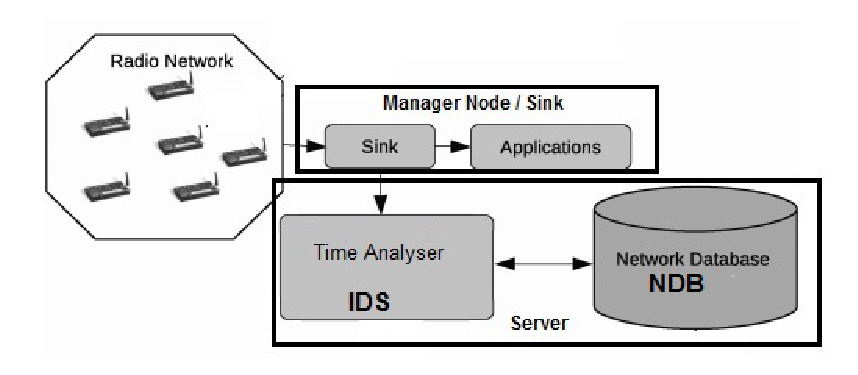
\includegraphics[width=0.5\textwidth]{IDS_fw}	
    \caption{IDS Framework}
    \label{fig:ids_fw}
\end{figure}
The IDS framework components has been shown in \ref{fig:ids_fw}.
The IDS has three kinds of components --- 
\begin{inparaenum}
\item the motes in the WSN that are subject to legitimate or illegitimate update; 
\item an IDS transport client (ITC) application that runs on the sink and works in coordination with the IDS to assists in intrusion detection; and
%The sink is protected from all kinds of security breaches whether it is physical or logical. 
\item an IDS application that runs on a system with higher computing resources which is physically attached to the sink, and houses a network database (NDB).
\end{inparaenum}
The chronology of the activities associated with the IDS  are shown in  \ref{fig:ids_fw}.
%%% <ashraf> strike out
%\begin{inparaenum}
%\item Updates are initiated using Deluge protocol;
%\item Deluge disseminates the new software image using the motes enroute to reach all the motes using a relay mechanism; 
%\item The nodes deliver their timing information to the sink using an AM packet;
%\item AM packets from the distant nodes rely on the other nodes enroute to reach the sink using a relay mechanism; and
%\item The ITC application in the sink delivers revelent information to the IDS for processing. 
%\end{inparaenum}
%The IDS analyses the acquired timing information to arrive at decision.
\begin{figure}[btp]
    \centering
    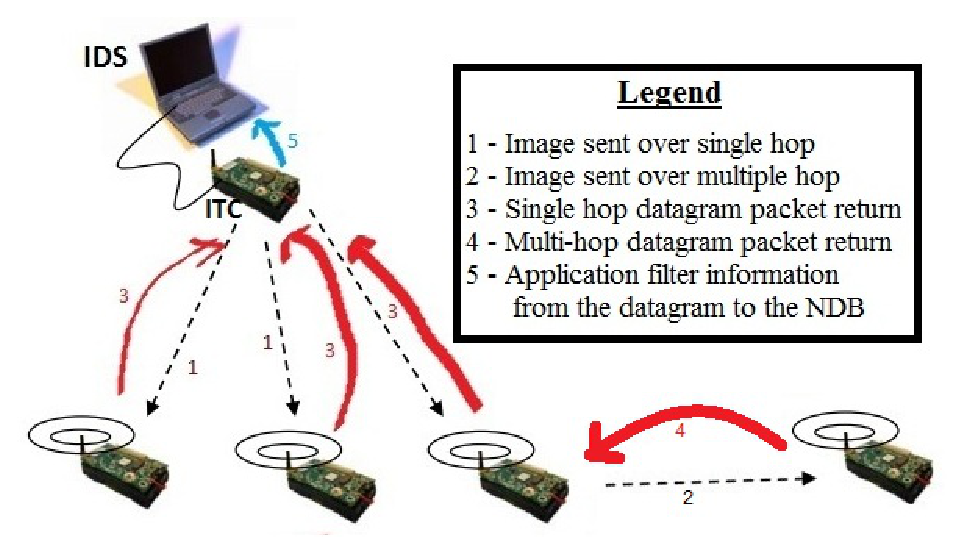
\includegraphics[width=0.5\textwidth]{IDS}
    \caption{IDS Modelling}
    \label{fig:ids_model}
\end{figure}

\subsubsection{Determining IWS}
\label{ssc:cal_iws}


%% <ashraf> We cannot go into these details in this paper; space limitation
The intrusion detection activity begins with the action of motes by endorsing update time and initiating AM to the sink. 
%An AM packet initiated for the IDS has several fields: destination address, type identifier that indicates the update time information and the protocol for IDS, timing information and a checksum value.
%[DO WE WANT TO INCLUDE THE PATH TAGGING; MAY BE LATER - IT INCREASES RELIABILITY, NOT DIRECTLY $IDS$ ACTIVITY?]
%[path tagging is good, but in all cases, what’s the risk from intruders messing with the reported data?]
%[PATH TAGGING CAN BE USED AS HEART-BEAT MESSAGE]
The packet travels to the sink using existing transport layer protocols.
%When it arrives at the sink, the checksum value is examined by the ITC to ensure that the packet content has not been altered enroute.
After checking for correctness, the ITC then inserts the update time, mote ID and related information to the NDB in the IDS.
The IDS maintains an identifier to differentiate among different update times from different runs for the same mote.
%
%The first software update run in the WSN is considered to be legitimate and the IDS takes this timing information as baseline.
%It is possible and desirable that the IDS is trained with several other update runs.
%More training improved the ability of the IDS to detect intrusion more accurately.
%Utilising multiple runs are useful and beneficial as it increases accuracy and dependency.
%However, the IDS needs to be manually controlled to enable multiple training runs.
%Outcome from these runs are statistically treated to build the baseline.

The authenticated initial software update runs are considered to be legitimate and the IDS takes this timing information as baseline.
The subsequent updates are liable to scrutiny by the IDS.
The timing analyser module in the IDS inspects the NDB once an update activity has been detected.
It determines the changes in the statistics of the update time and calculates IWS based on following utility function:

\begin{equation}
\label{eqn2} 
	\mathit{IWS} = \sum \limits_{i=0}^{n} \frac{\left| \mu_i - t_i \right|}{\sigma_i + 1}
%	f_1 = \sum\limits_{i=0}^{n} \left( \mu_i - t_i \right)
	\end{equation}
where, 
\begin{inparaenum}
\item $\mathit{i}$ --- Identification of the Mote;  
\item $\mathit{t_i}$ --- Image Update Time at Mote $\mathit{i}$; 
\item $\mathit{\mu_i}$ --- Mean Update Time at Mote$\mathit{i}$; 
\item $\mathit{\sigma_i}$ --- Standard Deviation of Update Time at Mote \emph{i} 
\end{inparaenum}	

\subsubsection{Building Intrusion Warning Zones}
\label{ssc:iw_zone}

Threshold for building of Intrusion Warning Zone (IWZ) depends on the assumed ability of the IDS having IWS knowledge of all possible intrusions in the network.
Such knowledge can be built by replicating intrusion activity from all nodes in the network once.
However, in case where it is not possible, replicating intrusion activity from the furthest few nodes may serve the purpose.
IDS can build a scale of possible expected range of IWS for the deployed topology and can classify the IWS in different zones to imply certain warning level.

The IDS considers an IWS upto 10\% from the scale to be safe and marks as `GREEN' zone, an IWS above 30\% to be possible intrusion and is marked as `RED' zone.
However, an IWS within the range of 10\% --- 30\% can neither be considered safe, nor an intrusion, hence is marked as `GREY' that indicates a situation where rules are not known.
However, the thresholds are not conclusive and may require some variation based on the density, power level used in the WSN and scale of deployment.

%% <Ashraf> We shall not include this portion in this paper
%\subsubsection{Database Structure}
%\label{ssc:db}
%The NDB stores the statistics of the update time of all the motes in the WSN for each update applied.
%It consists of three flat tables that performs as storage.
%The tables have been  designed to improve the IDS performance. 
%First, In-Network Activity Table (INT) consists of the  following fields:
%\begin{verbatim}
%mote_id, timestamp, id_seq, 
%upd_seq, upd_type, zone_type
%\end{verbatim}
%where, $mote\_id$ is the source node ID, $timestamp$ is the time when the new software image starts executing, $id_seq$ is the number of times an update arrived from same $mote\_id$, $upd\_seq$ is the number of time an update has been initiated from the sink.
%The unique key for INT is $mote\_id$, $upd\_seq$ pair.
%$upd\_type$ indicates if the record belonged to a baseline update.
%For a baseline update type, the $zone_type$ is zero, while for others it is updated to indicate if the update related to that particular mote from that particular run was processed as GREEN, GREY or RED.
%
%Secondly, the Baseline Table (BLT) holds the processed information from the legitimate runs and has the following fields:
%\begin{verbatim}
%mote_id, mu, sigma
%\end{verbatim}
%where, $mote\_id$ is the source node ID, $mu$ is the mean time and $sigma$ is the standard deviation for each $mote\_id$ from all legitimate runs.
%
%Finally, the Intrusion Activity Table (IAT) filters out necessary information from INT about most recent software update and contributes to the performance of the IDS.
%The table has two fields:
%\begin{verbatim}
%mote_id, timestamp
%\end{verbatim}
%where, $mote\_id$  and $timestamp$ are same as the corresponding fields in INT.
%Every time a decision on an update has been made and a new update is detected, this table is flashed.
%
%\subsubsection{Activities in the Network}
%\label{ssc:actnet}
%As part of enhancement into the Deluge protocol, the motes are enriched with the prior knowledge of the sink or sinks in the WSN.
%Whenever an update takes place in a mote, it reboots with the new software running and stores the bootup time in its memory.
%I NEED TO CONFIRM IF THE TIME IS ALREADY SAVED WITH THE IMAGE AS PART OF Deluge PROTOCOL IMAGE/GOLDEN IMAGE.
%The locally stored information  is used later in case it requires to recover from packet delivery failure.
%The information $type$, $mote\_id$,  $time\_stamp$,$upd\_seq$ are packed along with an additional checksum in an AM packet and forwarded to the sink/sinks.
%The AM has the following information in the packet:
%\begin{verbatim}
%|------------------------------------------|
%|Source|-----------------------------------|
%|  ID  |msgtype|timestamp|upd_seq|checksum||
%|------|-----------------------------------|
%
%Figure: Need to draw a better picture
%\end{verbatim}
%The AM packet is relayed through the network to the sink.
%
%\subsubsection{Activities in the Sink}
%\label{ssc:actsink}
%As an AM arrives from the radio network to the sink, the ITC application running on the sink verifies the checksum.
%If the checksum fails, the packet is discarded and failure recovery is initiated once only in coordination with the IDS.
%However, if the AM passes checksum, the ITC application extracts the relevant information and populates the INT in the resident host system. 
%
%\subsubsection{Activities in the IDS}
%\label{ssc:actids}
%An update is typically initiated from the host system where the IDS resided.
%The IDS constantly monitors the programming port and coordinates with the ITC. 
%They automatically identify the first update as input for baseline training data.
%It is possible to put the IDS in training mood for extended number of updates.
%Result from all updates run during the training period are statistically treated to build the baseline.
%Though the IDS can work theoretically with a single update, it is recommended to have minimum three updates for the training phase while running more training updates is desirable.
%For our experiments, we have considered 20 runs for each topology.
%
%Once the training phase ends, the IDS calculates mean and standard deviations at each of the motes and stores the  information on BLT.
%It also stores the number of update runs it considered for the BLT.
%This number contributes two folds:
%\begin{inparaenum}
%\item it indicates the reliability of the training data / baseline; and
%\item the number is used for statistical processing in case there is a need to increase the training data at a later time or data from an update is identified as acceptable is automatically included in baseline computation and the BLT is updated.
%\end{inparaenum}
%Once the BLT has been built, the IDS runs on active mood and all updates are subject to intrusion checks.
%When an update is initiated in the WSN, data pushed into the INT are filtered and relevant information related to the ongoing update populates the  IAT.
%The IDS waits upto a specific time, which is determined by the maximum time taken to complete a network-wide  update during the training phase, before it reports the findings about intrusion possibility.
%While the procedure described above is quite straight forward, it gets complicated because of the unreliable packet transmission pattern experienced by WSN due to node failure, link failure and node reboot \cite{aro04}, \cite{bec04}.
%IDS reports the findings with a provision of updating it later when an expected data from certain mote are not available within reasonable time.
%In such case, the IDS employs a packet recovery mechanism to obtain necessary information.
%
%The packet recovery mechanism is initiated when a valid packet is not available form one or more motes within  the  determined maximum time from the updates  during the training phase.
%Upon receiving signal from the IDS, the ITC initiates AM to the specific requesting a retransmission of the update time and waits further  triple time for the required AM packet. If the packet is available,  IWS is recomputed and decision is updated accordingly.
%If the packet is still not available within specified time, the node is marked as compromised or failed and a notification is generated.
%
%

\section{Results and Evaluation}
\label{sec:eval}

\begin{table*}[t!]
\centering
\begin{tabular}{|l|*{20}{r|}r}
\hline
\bd{Node ID}           & \bd{1} & \bd{2} & \bd{3} & \bd{4} & \bd{5} & \bd{6} & \bd{7} & \bd{8} & \bd{9} & \bd{10} & \bd{11} & \bd{12} & \bd{13} & \bd{14} & \bd{15} & \bd{16} & \bd{17} & \bd{18} & \bd{19} & \bd{20} \\
%Mote ID           & 1 & 2 & 3 & 4 & 5  & 6 & 7 & 8 & 9 & 10 & 11 & 12 & 13 & 14 & 15  & 16 & 17 & 18 & 19 & 20 \\
\hline
$\mu$            & 0 &19 & 19& 69&139 &213&276&344&377&432 &432 &432 &377 &335 &273 & 207&137 & 68 & 17 & 19 \\
$\sigma$		 & 0 & 5 & 5 & 6 & 22 & 36& 37&43 &44 & 44 & 44 & 44 & 44 & 45 & 44  & 33 & 24 & 5 & 3 & 5 \\
\hline
\end{tabular}
\caption{Time statistics of motes in Elliptical topology}
\label{tab:stat_ellip}
\end{table*}

\begin{table*}[t!]
\centering
\begin{tabular}{|l|*{20}{r|}r}
\hline
\bd{Node ID}           & \bd{1} & \bd{2} & \bd{3} & \bd{4} & \bd{5} & \bd{6} & \bd{7} & \bd{8} & \bd{9} & \bd{10} & \bd{11} & \bd{12} & \bd{13} & \bd{14} & \bd{15} & \bd{16} & \bd{17} & \bd{18} & \bd{19} & \bd{20} \\
\hline
$\mathit{IWS}$
                 &0.01&16 &19 &73 & 140 &203 &246 &336 &344 &396 &395 &535 &406 &332 &269 &237 &113 & 72& 16 & 16 \\
\hline
\end{tabular}
\caption{Mote IWS in Elliptical topology. Further explained in Figure~\ref{fig:ellip}}
\label{tab:iws_ellip}
\end{table*}

\begin{figure*}[t!]
\label{fig:ellip}
    \centering
    \begin{subfigure}[b]{0.5\textwidth}
        \centering
        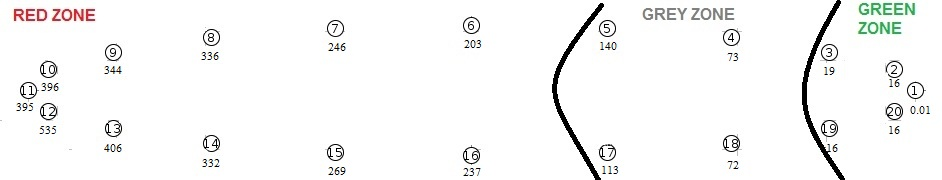
\includegraphics[height=1in, width=4in]{Elliptical}
        \label{subfig:elliptopo}
        \caption{IWS and Relative position of nodes}
    \end{subfigure}%
    ~ 
    \begin{subfigure}[b]{0.5\textwidth}
        \centering
        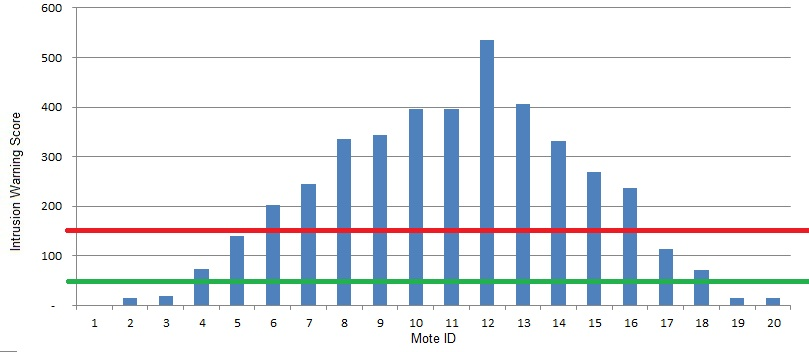
\includegraphics[height=1.2in]{Elliptical_column}
        \label{subfig:ellipgraph}
        \caption{Comparison of IWS at different motes}
    \end{subfigure}
    \caption{Relative position and comparison of IWS for intrusion at different motes from data in Table~\ref{tab:iws_ellip}}
\end{figure*}

In this section, we presents the data found in the course of this investigation, their interpretation and evaluate the contribution.
While discussing the performance and effects of the proposed IDS in different topologies are useful, we shall concentrate our discussion on results and findings elliptical topology only.
Discussing any of the topologies presents fair idea about the outcomes from the others. 
We shall mention the cases when the outcome was considered to be exception and contrary to the expectations.
The space requirement also motivates us to limit the discussion to necessary details only.
%\notedme{Is it closest to what you see in other papers? I'd not have thought so, in which case I'd think you need to justify why you're focusing on it... Also, there's unnecessary text repetition here.}
%% <Ashraf> The discussion is taken this way because of the spacew limitation and otherwise introducing all the results would be repeatation of the same thing, I guess. I'll look for papers that describe similar things.

%\subsection{Data1 + Discussion}

% We have selected data from elliptical topology for several reasons.
% Ellipse has a shape which is almost midway among the range of topologies between a circular and a linear one.
% Extending the minor axis of the ellipse makes the topology equivalent to a circle, while contracting it is equivalent to a grid or even a linear topology.
% Thickening the perimeter of the circle turns it into a double ring.
% Again, the linear topology can be considered as a tree with one or two branches.
% Extending it with more branches presents a fairly complex tree structure.
% Because of these similarities, discussing elliptical topology is an interesting choice.
%\notedme{Maybe...}
%% <Ashraf> removed because of space

The ellipse shaped deployment of 20 nodes, shown in Figure~\ref{subfig:elliptopo}, has been designed considering several requirements.
The motes on either side of minor axis remained within each others' transmission range, whereas motes on the either side of the major axis did not.
%Total 20 nodes were deployed with the minor axis being 30 meter and the major axis being way larger than that.
The transmission power level was set at 100\%. 
% which allowed a  transmission range of 50 meter and nodes were  able to interfere other nodes at  up to 100 meter apart.
The motes were placed at a spacing of 35 meters along the circumference of the ellipse to enable multiple transmission paths to all the motes.
It contributed to achieve  redundancy and  reliable image transfer. 

%The simulations proceeded without interruption and produced expected results.
% \notedme{This makes it sound like you're not going to present the results, which would be bad.}
% To build the baseline data, we assigned mote ID 1 as the sink and ran 20 updates initiated from the sink.
% The output from these runs were processed as describes in Section~\ref{ssc:build_baseline} and were statistically treated to compute the mean and standard deviation of the  time at which each of the nodes were updated with the new image.
%The computation results have been presented in Table~\ref{tab:stat_ellip}.
%\notedme{not yet clear enough what this table contains. Presumably `Node ID' should be explained to be the ID of the node from which to simulate injecting a malicious update so as to calculate the IWS? (+ broken ref)}
%% <Ashraf> restructured
Table~\ref{tab:stat_ellip} shows the statistical measurements obtained at different motes.
The first row in Table~\ref{tab:stat_ellip} contain the Node IDs that are headers for the data displayed underneath.
Node ID indicates the identification of each node in the deployment.
The next two rows describe the baseline data i.e., mean and standard deviation computed from the 20 legitimate updates initiated from the sink.
Analysing the baseline data shows that update time of the motes further away from the sink have higher mean and standard deviation.  
However, standard deviation raises gradually, though it varies little for relatively small distance difference when multiple paths are present.
The the stability of standard deviation results from availability of redundant paths, which makes the image transfer more efficient and reliable.
Therefore, even remaining at considerably different distances from the sink, mote ID 8, 9, 10, 11, 12, 13, 14 and 15  have quite similar standard deviation of update time.
In contrast to this, mean increases sharply as the motes are placed further from the sink.
The result in baseline data shows that motes closer to the sink have lower mean which increases sharply with the increase in distance.

Results obtained from these simulated intrusions are reported in Table~\ref{tab:iws_ellip}.
Cells in the last row contain the IWS calculated using  the utility function shown in Equation~\ref{eqn2} for the test runs initiated from the node indicated at top of the column.
Each of the motes were considered as intrusion point to measure IWS.
It can be clearly seen that IWS at different motes differ considerably.
The data shown in the table can best be interpreted when related to Figure~\ref{fig:ellip}, which shows defined zones and IWS measured when intrusion was initiated at different motes.
Figure~\ref{subfig:elliptopo} shows the actual relative positions of the motes with mote ID written at the centre of the tiny circle and IWS measured when an intrusion attempt has been initiated from the mote. 
The figure additionally divides the region in GREEN, GREY and RED zones according to the technique discussed in Section~\ref{ssc:actids}.
The graph in  Figure~\ref{subfig:ellipgraph} shows the relative measures of the IWS from the motes.

IWS shown in Table~\ref{tab:iws_ellip} were used to build a scale that ranged from $0$ to maximum of $\mathit{IWS}$.
Building this scale was crucial for the ability to classify the IWS to meaningful zones.
%\notedme{I thought that there were difficulties determining these zones?}
%% <Ashraf> I am not sure. Do you consider this description too simple?
However, it is not possible to build the scale without the knowledge of the expected IWS from the furthest nodes in the network.
Nevertheless, we established two threshold levels at 10\% and at 30\% that were useful in zone classification using intuitive heuristics.
Details of the zoning has been discussed in Section~\ref{ssc:iw_zone}.


%\section{Discussion}

The utility function presented in Equation~\ref{eqn2} is designed to neutralise the undesired %/unexpected
changes in mean and standard deviation which are expected to contribute to a near zero IWS.
%\notedme{zero is just an English word. Why are you typesetting it differently? NB: if you were to typeset it in maths, this is not the correct way to do so: \LaTeX doesn't know that you mean zero to be a word, and thus will instead typeset it as a product of individual variables z, e, r, o, ...}
%% <Ashraf> Addressed 
A near zero IWS is further classified as GREEN zone to indicate a legitimate software update. 

The IWS increases linearly with the increase in distance from the sink.
The `distance' term can be misleading in the context of our discussion and demands further clarification.
Euclidean distance between a mote and the sink does not make useful sense as the packets in the network must travel using a relay mechanism through other motes in the network.
Because of the availability of the multiple paths, it is not possible to quantify the exact distance that a packet would travel while transporting form a mote to the sink.
However, an estimation of distance along the most probable link path based on the connectivity may be considered.

IWS is considerably higher for intrusion at distant motes than ones which are close to the sink.
This phenomena is topology dependent, which also implies  that it is connectivity dependent.
It is possible that if IWS in a network are organised in a specific order, it would represent/resemble   the original topology in some fashion.
For example, in the elliptical topology, the link path between node 1 and node 11 through node 5 is represented by a curve with a positive slope or rise.
On the other hand, the link path through node 15 is represented by a fall or a negative sloped curve.
There is a relationship between the curvature/eccentricity of the original topology and the represented curve or  trend.
%This implication would be more evident once we discuss more topologies in the upcoming paragraphs. {Only if we discuss the other topologies}.
However, establishing the relationship is beyond the scope of this paper.

%\subsection{discussion of contributions}


\begin{table*}[t!]
\centering
\begin{tabular}{|l|*{20}{r|}r}
\hline
\bd{Node ID}           & \bd{1} & \bd{2} & \bd{3} & \bd{4} & \bd{5} & \bd{6} & \bd{7} & \bd{8} & \bd{9} & \bd{10} & \bd{11} & \bd{...} & \bd{31} & \bd{32} & \bd{33} & \bd{34} & \bd{35} & \bd{36} & \bd{37} & \bd{38} \\
%Mote ID           & 1 & 2 & 3 & 4 & 5  & 6 & 7 & 8 & 9 & 10 & 11 & ...& 31 & 32 & 33  & 34 & 35 & 36 & 37 & 38 \\
\hline		\hline

Power	  &  &  &  &  &  &  &  &  &  &  &  &  &  &  &   &  &  &  &  &  \\
$100\% $          & 512 & 529 & 512 & 512 & 512  & 512 & 476 & 478 & 476 & 459 & 458 & ...& 49 & 47 & 53  & 48 & 49 & 51 & 47 & 29 \\
\hline

Power	  &  &  &  &  &  &  &  &  &  &  &  &  &  &  &   &  &  &  &  &  \\
$50\%$            &31 & 59&254& 31& 31 &283& 32& 32& 254& 31 &253 & ...& 31 & 31 & 31  & 30 & 31 & 31 & 30 & 0 \\
\hline
\end{tabular}
\caption{IWS from intrusion at motes in `Owheo Sensor Network'. Further explained in Figure~\ref{fig:owheo}}
\label{tab:owheo}
\end{table*}


\begin{figure*}[t!]
\label{fig:owheo}
    \centering
    \begin{subfigure}[b]{0.5\textwidth}
        \centering
        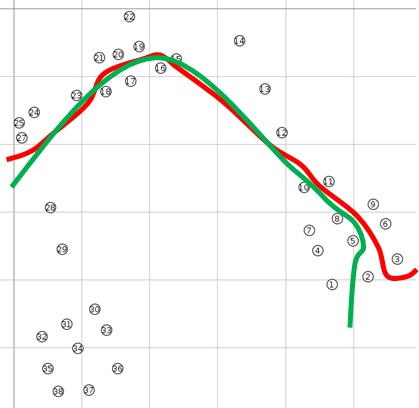
\includegraphics[height=2.5in]{Owheo_full}
        \label{subfig:owheo_full}
        \caption{Zone boundary at Full Power Level}
    \end{subfigure}%
    ~ 
    \begin{subfigure}[b]{0.5\textwidth}
        \centering
        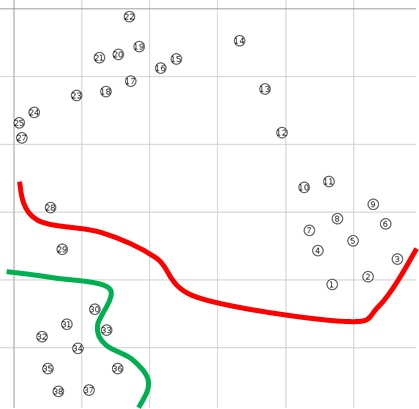
\includegraphics[height=2.5in]{Owheo_half}
        \label{subfig:owheo_half}
        \caption{Zone boundary at Half Power Level}
    \end{subfigure}
    \caption{Comparison of Zone boundary for power level variations in `Owheo Sensor Network'. IWS of the motes at the power levels are shown in Table~\ref{tab:owheo}}
\end{figure*}

The main contribution of this research project comes from the fact that the IDS is able to report an anomaly from a software update in quantitative term like the IWS.
For example:  a regular legitimate update, initiated from node ID 1, resulted into a IWS of 0.01.
The result matched the theoretical expectation of a near zero IWS.
In addition to this, when intrusion scenario were simulated from the nodes near the sink, the IWS reported was fairly low, e.g. 16 for mote ID 2, 19, and 20
 and 19 for node 3 
 and likewise.
Because of the fact that IWS of the motes close to the sink are likely to be very low, which is in line with the theoretical expectation, it is quite difficult to conclude if such a IWS indicate an intrusion. 
However, for the distant motes, the IWS is quite high and the IDS can conclude such cases as intrusion, e.g. IWS of 246 for mote ID 7, 269 for mote ID 15, 395 for mote ID 11, 535 for mote ID 12 and likewise indicate intrusion.


While reporting severity or likelihood of an intrusion in quantitative term like the IWS is useful, it is more beneficial if the quantity is associated with some kind of interpretation.
The technique of associating such interpretation has been discussed in Section~\ref{ssc:iw_zone} and in this Section. 
In the elliptical topology intrusion scenario, maximum IWS reported in the presented data in Table~\ref{tab:iws_ellip} was 535. 
Motes reporting 10\% of maximum IWS i.e., an IWS up to 53.5 would be considered in the GREEN zone.
%\notedme{Why is this the IWS value for green? You've not explained.}
%% <Ashraf> addressed
For example, in figure~\ref{subfig:elliptopo}, mote ID 2, 3, 19, and 20 are in this zone.
On the other hand, IWS above 53.5 and bellow 160.5, which is 10\% -- 30\% of the maximum, are considered to be in the GREY zone. 
Motes in this zone are 4, 5, 17, and 18.
They can neither be considered free from intrusion, nor it is possible to easily arrive at a decision that the scores indicate intrusion for sure.
In contrast to both the scenarios describes above, IWS above 160.5, which is beyond 30\% of the maximum, is considered to be an intrusion.
All other motes in the topology have a IWS above this threshold level and hence are considered to be more easily detectable by the IDS. %\notedme{Eh? How does this follow?} %% <Ashraf> addressed

The idea of zoning associated with the IWS is very beneficial in securing a WSN.
It is useful in designing a secure network deployment, which is considered to be another major contribution of the research work.
%\notedme{`immensely' is too over the top.} %% <Ashraf> `immensely' removed
The motes which are found to be in the GREEN zone must be adequately secured by design with additional physical security as intrusion in these motes are not observed by the IDS.
%\notedme{OK, yep---I like this.} %% <Ashraf> addressed
On the other hand, motes in the GREY zone need additional monitoring which would aid determining if the IWS indicated a real intrusion or a false positive.
The additional monitoring could be in the form of an algorithmic or physical observation or listening post or even employing additional protocol.
The rest of the region, identified by the RED zone, is under the effective surveillance of the IDS and the IDS is expected give a reliable estimation of correct behaviour in this region.
%\notedme{not secure really, but yes, where the IDS can give a reliable estimation of correct behaviour}

The concept of zoning using the IDS is a very useful tool in designing secure WSN deployment.
A network is more secure when it has a smaller GREEN and GREY zone.
A smaller GREEN zone implies the requirement of lesser resources to impenetrably secure less number of motes.
Similarly, a smaller or non-existent GREY zone would require lesser monitoring measures.
Such a secure WSN can be designed by physically relocating some of the motes or even by varying the factors like power level.
However, obtaining real world scenario by varying different sets design parameters e.g., power levels, position of nodes, etc is an impossible task for even a small WSN.
The simulation environment used to design IDS can be effectively utilised to obtain expected IWS score range, and rank the sets based on how effectively they produce IWS values. 
For example, we have simulated the IWS scenario of the `Owheo Sensor Network' at two different power levels in our quest to design a secure WSN using the IDS.
`Owheo Sensor Network', which is the WSN deployed in the Department of Computer Science building at the University of Otago, is intended to be used for research purposes.
%\notedme{I don't think you're quite stating the contribution clearly enough yet: that for different sets of potential design parameters for the WSN (e.g. power levels, position of nodes, etc.) you would be able to simulate the IWS score range, and rank the sets based on how effectively they produce IWS values. For example, it's not clear that your shift into discussing the zones is just an indirect way of discussing the underlying IWS scores.}
%% <Ashraf> addressed

Table~\ref{tab:owheo} shows the IWS at different motes as intrusion points at 100\% and 50\% power levels. 
In `Owheo Sensor Network', mote ID 38 was marked as the sink and mote ID 26 does not exist.
At 100\% power level, 19 nodes (mote ID 1, 4, 5, 7, 8, 10, 16, 17, 18, 28, 29, 30, 31, 32, 33, 34, 35, 36, and 37) were in GREEN zone, only one node (mote ID 2) was in GREY zone and the rest 16 nodes were in RED zone.
The deployment and the zoning boundaries at 100\% power level has been shown in Figure~\ref{subfig:owheo_full}.
When the same deployment was simulated at 50\% power level, only seven nodes (mote ID 30, 31, 32, 34, 35, 36, and 37) were in GREEN zone, two nodes (mote ID 29, and 33) were in GREY zone and rest 27 motes were in RED zone.
The deployment and the zoning boundaries at 50\% power level has been shown in Figure~\ref{subfig:owheo_half}.
Comparing the scenarios presented in  Figure \ref{subfig:owheo_full} and \ref{subfig:owheo_half}, it can clearly be established that Figure~\ref{subfig:owheo_half}, i.e. deployment at 50\% power level is more secure than the other because of two reasons:
\begin{inparaenum}
\item it has a smaller sized GREEN and GREY zone; and 
\item there are fewer nodes in these zones. 
\end{inparaenum}
The deployment can be made more secure by physically relocating some of the motes from GREEN zone to RED zone, provided the relocation does not hamper the original intended purpose of the WSN.
However, any change in topology or design parameters like power level will require recalibrating the IDS from the beginning. 
%\notedme{I like this paragraph up to the last sentence. The last sentence doesn't make sense necessarily, since it seems to suggest that you can just move nodes directly between the zones. However any change in topology will require recomputing the zones, and they will change, potentially significantly...}
%% <Addressed>


%Identifying node failure and node compromise
The IWS is also able to detect node failures in the WSN.
%This additional advantage comes as a by-product contribution.
%However, as this was not a design consideration, the contribution is not robust enough, yet it is worth mentioning.
%\notedme{You've talked about this meta-point too much, now.}
%% <Ashraf> Actually, a `not' before `robust' went missing. :)
The case of a node not reporting its update time within a specified delay is handled by a error recovery procedure put in place by the IDS.
If the recovery procedure fails, the node is considered to have failed or have been compromised.
A unusual update time chronology and resulting unusual IWS  indicates the probability of some other types of attacks in WSN like node relocation, node repudiation, node compromise, not just a transient failure whihc is something worth paying attention to.
% However, such failure resulting into contribution towards an IWS which is quite different for the update pattern detected from the timing information reported by the other nodes.
% The IDS structure is such that it has an expected pattern and shape of IWS for an intrusion at some specific point.
% If the shape is distorted to a great extent, it indicates some unusualness which can be attributed to some other phenomena like node failure or compromise.
% The node failure or node compromise can take place concurrently with or without intrusion.
% It might also indicate a different type of attack associated with a physical intrusion.
% An interpretation form the IDS view of the topology would enable identification of some other types of attacks in WSN like node relocation, node repudiation, node compromise.
% \notedme{This paragraph probably needs to be much shorter. The point is simply that you're looking for a timing pattern, and that it involves a fair few transmissions. Thus if you see an anomaly, given that you're already comparing against a statistical distribution, it's probably not just a transient failure, and thus something worth paying attention to.}
%%<Ashraf> addressed


In this paper, we have modelled a IDS solution to one of the weaknesses in WSN that can be capitalised by an adversary to invalidate a mission critical deployment of the technology in robotics. 
The proposed system watches over the software update pattern for over the air update protocol in WSN, computer an IWS that can quantitatively indicate a possible intrusion.
In addition to this, the IDS environment can be used to design a secure WSN deployment.
The IDS also can indicate some other kinds of anomalies such as node relocation, node repudiation, node compromise and so on.
In future,  the IDS can be implemented to examine testbed performance including cases of multiple sink with mobile sensors which would be very useful in robotics applications.

%\subsection{Discuss other topologies}

%Not included in this paper. Already long enough.
%Insight for secure deployment. which topologies would work better - idea
%Insight for a deployment that would ensure better connectivity
%
%
%Interpretation of the results.
%Our argument in support of the results.
%
%Explanation of the results to answer the question - so what.
%Why the result was important.
%Why does this matter .

%Constraints and limitations of the program
%Opportunities for future work

% Must explicitly state what is my contribution
% If there are some recommendations, must include them here
%What are my specific contributions to the academic society?
%Do I have some recommendations about it?



% \section{Conclusion}
 % \label{sec:concl}


%\begin{figure}[!t]
%\centering
%\includegraphics[width=2.5in]{myfigure}
% where an .eps filename suffix will be assumed under latex, 
% and a .pdf suffix will be assumed for pdflatex; or what has been declared
% via \DeclareGraphicsExtensions.
%\caption{Simulation Results}
%\label{fig_sim}
%\end{figure}

% An example of a double column floating figure using two subfigures.
%\begin{figure*}[!t]
%\centerline{\subfloat[Case I]\includegraphics[width=2.5in]{subfigcase1}%
%\label{fig_first_case}}
%\hfil
%\subfloat[Case II]{\includegraphics[width=2.5in]{subfigcase2}%
%\label{fig_second_case}}}
%\caption{Simulation results}
%\label{fig_sim}
%\end{figure*}
% Note that often IEEE papers with subfigures do not employ subfigure
% captions (using the optional argument to \subfloat), but instead will
% reference/describe all of them (a), (b), etc., within the main caption.

% An example of a floating table. Note that, for IEEE style tables, the 
% \caption command should come BEFORE the table. Table text will default to
% \footnotesize as IEEE normally uses this smaller font for tables.
% The \label must come after \caption as always.
%
%\begin{table}[!t]
%% increase table row spacing, adjust to taste
%\renewcommand{\arraystretch}{1.3}
% if using array.sty, it might be a good idea to tweak the value of
% \extrarowheight as needed to properly center the text within the cells
%\caption{An Example of a Table}
%\label{table_example}
%\centering
%% Some packages, such as MDW tools, offer better commands for making tables
%% than the plain LaTeX2e tabular which is used here.
%\begin{tabular}{|c||c|}
%\hline
%One & Two\\
%\hline
%Three & Four\\
%\hline
%\end{tabular}
%\end{table}
% Note that IEEE does not put floats in the very first column - or typically
% anywhere on the first page for that matter. Also, in-text middle ("here")
% positioning is not used. Most IEEE journals/conferences use top floats
% exclusively. Note that, LaTeX2e, unlike IEEE journals/conferences, places
% footnotes above bottom floats. This can be corrected via the \fnbelowfloat
% command of the stfloats package.

%\section*{Acknowledgment}
% trigger a \newpage just before the given reference
% number - used to balance the columns on the last page
% adjust value as needed - may need to be readjusted if
% the document is modified later
%\IEEEtriggeratref{8}
% The "triggered" command can be changed if desired:
%\IEEEtriggercmd{\enlargethispage{-5in}}

% references section
\bibliographystyle{IEEEtran}
\bibliography{icara}



% that's all folks
\end{document}


